\documentclass{standalone}
\usepackage{tikz}
\usetikzlibrary{patterns, positioning}
\usepackage[sfdefault]{ClearSans} %% option 'sfdefault' activates Clear Sans as the default text font
\usepackage[T1]{fontenc}

\begin{document}
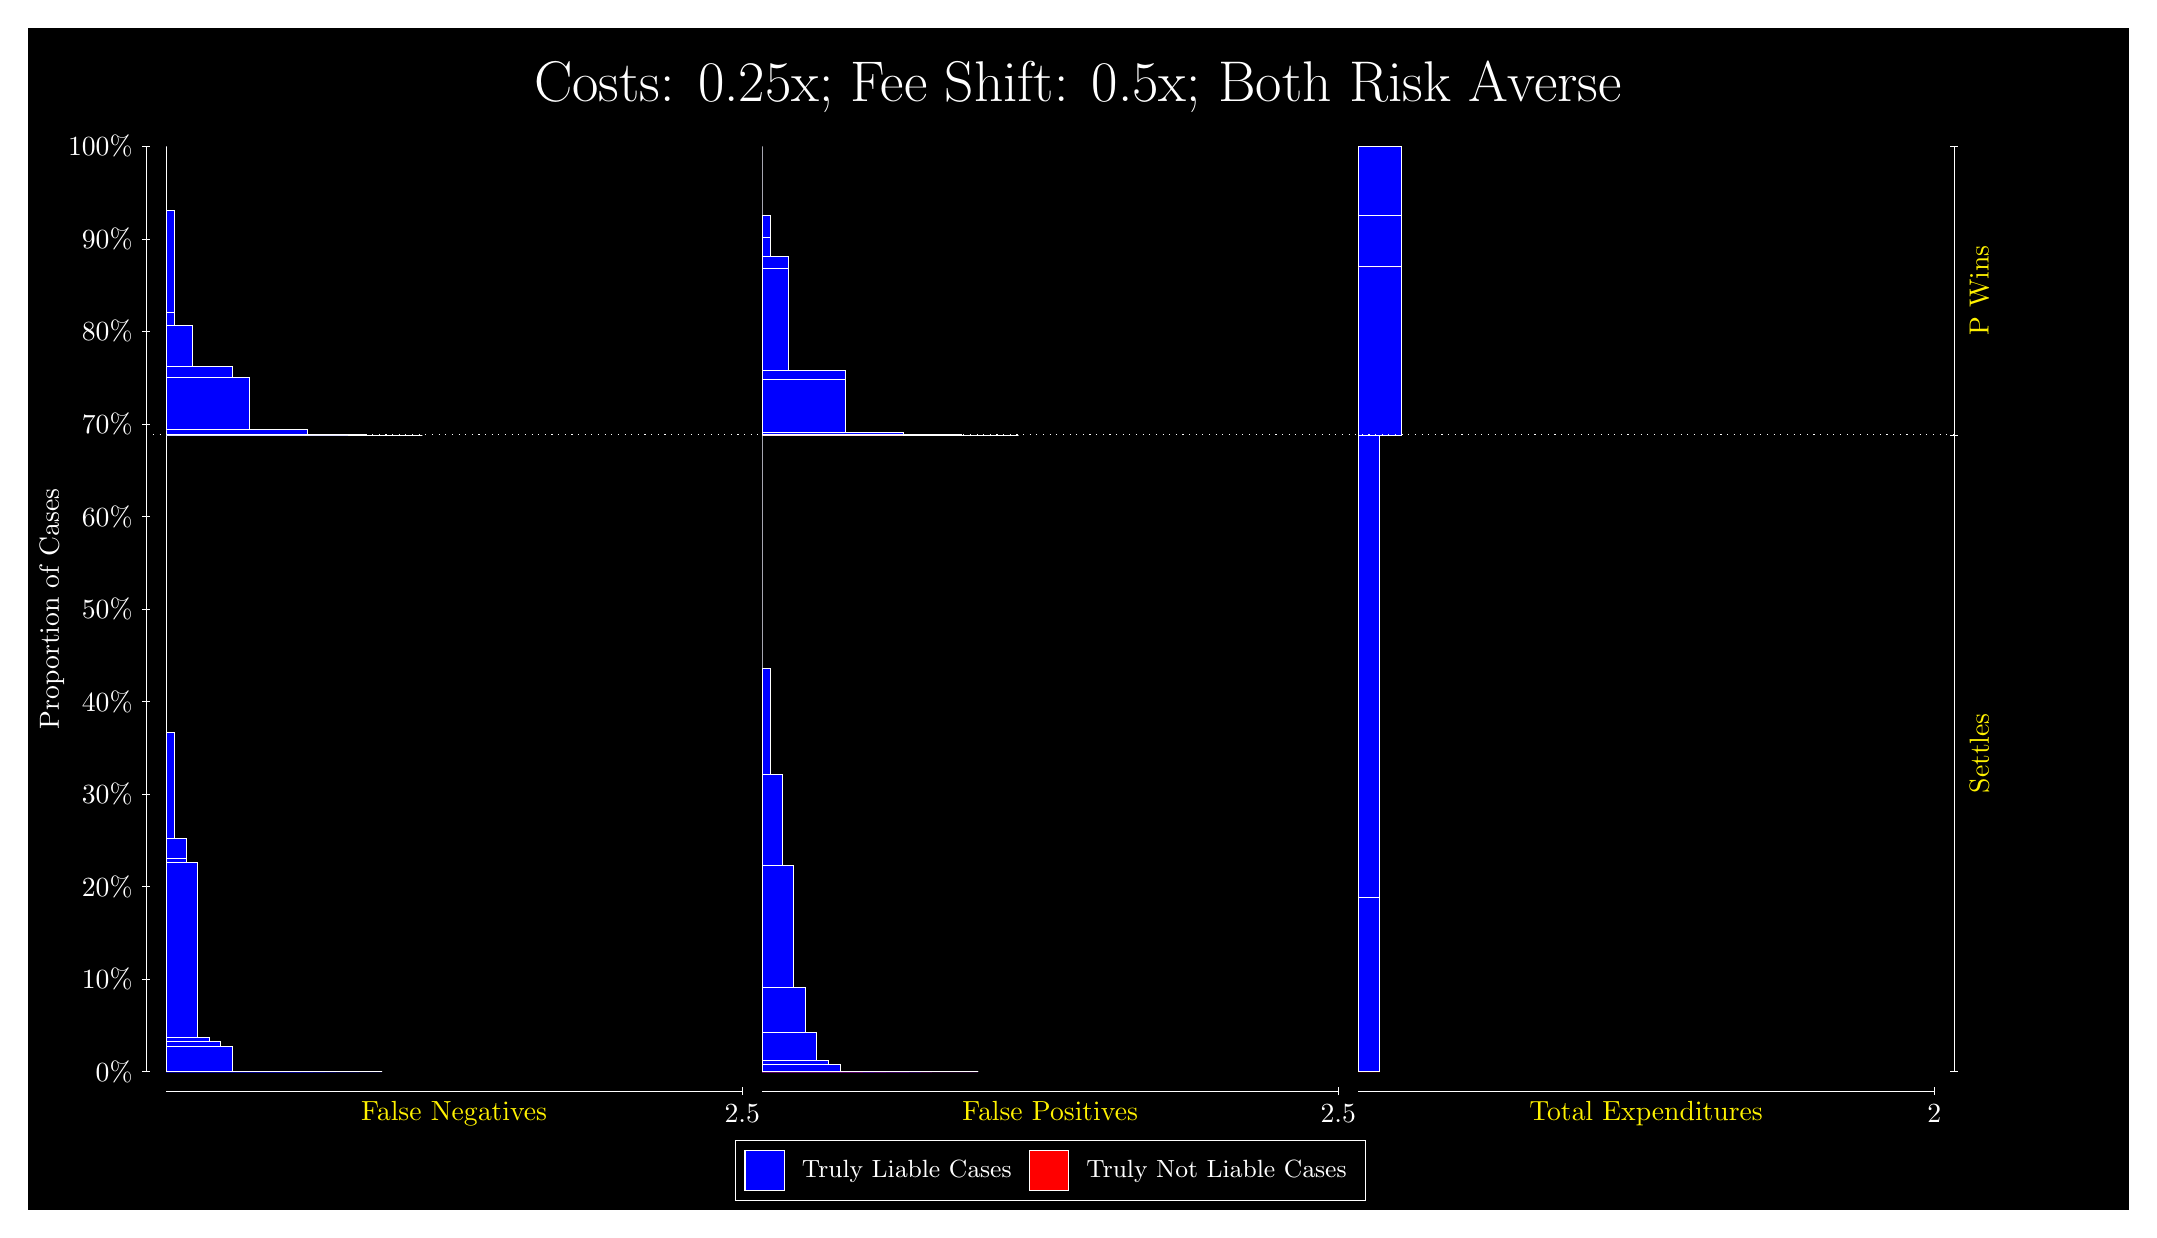
\begin{tikzpicture}
\draw[fill=black] (0,0) rectangle (26.667,15);
\draw[text=white] (0,13.5) rectangle (26.667,15) node[midway] {\huge Costs: 0.25x; Fee Shift: 0.5x; Both Risk Averse};
\draw[white, very thin] (1.5,1.75) -- (1.5,13.5);
\node[rotate=90, text=white, anchor=center] at (0.3, 7.625) {Proportion of Cases};
\draw[white, very thin] (1.45,1.75) -- (1.55,1.75);
\node[text=white, anchor=east] at (1.45, 1.75) {0\%};
\draw[white, very thin] (1.45,2.925) -- (1.55,2.925);
\node[text=white, anchor=east] at (1.45, 2.925) {10\%};
\draw[white, very thin] (1.45,4.1) -- (1.55,4.1);
\node[text=white, anchor=east] at (1.45, 4.1) {20\%};
\draw[white, very thin] (1.45,5.275) -- (1.55,5.275);
\node[text=white, anchor=east] at (1.45, 5.275) {30\%};
\draw[white, very thin] (1.45,6.45) -- (1.55,6.45);
\node[text=white, anchor=east] at (1.45, 6.45) {40\%};
\draw[white, very thin] (1.45,7.625) -- (1.55,7.625);
\node[text=white, anchor=east] at (1.45, 7.625) {50\%};
\draw[white, very thin] (1.45,8.8) -- (1.55,8.8);
\node[text=white, anchor=east] at (1.45, 8.8) {60\%};
\draw[white, very thin] (1.45,9.975) -- (1.55,9.975);
\node[text=white, anchor=east] at (1.45, 9.975) {70\%};
\draw[white, very thin] (1.45,11.15) -- (1.55,11.15);
\node[text=white, anchor=east] at (1.45, 11.15) {80\%};
\draw[white, very thin] (1.45,12.325) -- (1.55,12.325);
\node[text=white, anchor=east] at (1.45, 12.325) {90\%};
\draw[white, very thin] (1.45,13.5) -- (1.55,13.5);
\node[text=white, anchor=east] at (1.45, 13.5) {100\%};

\draw[white, very thin] (24.457,1.75) -- (24.457,13.5);
\draw[white, very thin] (24.407,1.75) -- (24.507,1.75);
\node[anchor=west] at (24.407, 1.75) {};
\draw[white, very thin] (24.407,9.8365) -- (24.507,9.8365);
\node[anchor=west] at (24.407, 9.8365) {};
\draw[white, very thin] (24.407,13.5) -- (24.507,13.5);
\node[anchor=west] at (24.407, 13.5) {};

\draw[white, very thin, fill=blue] (1.75,1.75) rectangle (4.4946,1.75);
\draw[white, very thin, fill=blue] (1.75,1.75) rectangle (4.2018,1.75);
\draw[white, very thin, fill=blue] (1.75,1.75) rectangle (3.9091,1.75);
\draw[white, very thin, fill=blue] (1.75,1.75) rectangle (3.7627,1.75);
\draw[white, very thin, fill=blue] (1.75,1.75) rectangle (3.6163,1.75);
\draw[white, very thin, fill=blue] (1.75,1.75) rectangle (3.4699,1.75);
\draw[white, very thin, fill=blue] (1.75,1.75) rectangle (3.3236,1.7507);
\draw[white, very thin, fill=blue] (1.75,1.7507) rectangle (3.1772,1.7507);
\draw[white, very thin, fill=blue] (1.75,1.7507) rectangle (3.0308,1.7507);
\draw[white, very thin, fill=blue] (1.75,1.7507) rectangle (2.8844,1.7534);
\draw[white, very thin, fill=blue] (1.75,1.7534) rectangle (2.738,1.757);
\draw[white, very thin, fill=blue] (1.75,1.757) rectangle (2.5917,2.0683);
\draw[white, very thin, fill=blue] (1.75,2.0683) rectangle (2.4453,2.1291);
\draw[white, very thin, fill=blue] (1.75,2.1291) rectangle (2.2989,2.1879);
\draw[white, very thin, fill=blue] (1.75,2.1879) rectangle (2.1525,4.4022);
\draw[white, very thin, fill=blue] (1.75,4.4022) rectangle (2.0062,4.4605);
\draw[white, very thin, fill=blue] (1.75,4.4605) rectangle (2.0062,4.7136);
\draw[white, very thin, fill=blue] (1.75,4.7136) rectangle (1.8598,6.0612);
\draw[white, very thin, fill=red] (1.75,6.0612) rectangle (1.75,6.0612);
\draw[white, very thin, fill=blue] (1.75,6.0612) rectangle (1.75,9.8365);
\draw[white, very thin, fill=blue] (1.75,9.8365) rectangle (5.0069,9.8365);
\draw[white, very thin, fill=blue] (1.75,9.8365) rectangle (4.275,9.8375);
\draw[white, very thin, fill=blue] (1.75,9.8375) rectangle (4.0554,9.8375);
\draw[white, very thin, fill=blue] (1.75,9.8375) rectangle (3.5431,9.9028);
\draw[white, very thin, fill=blue] (1.75,9.9028) rectangle (3.3236,9.9028);
\draw[white, very thin, fill=blue] (1.75,9.9028) rectangle (2.8112,10.571);
\draw[white, very thin, fill=blue] (1.75,10.571) rectangle (2.5917,10.708);
\draw[white, very thin, fill=blue] (1.75,10.708) rectangle (2.0793,11.231);
\draw[white, very thin, fill=blue] (1.75,11.231) rectangle (1.8598,11.389);
\draw[white, very thin, fill=blue] (1.75,11.389) rectangle (1.8598,12.682);
\draw[white, very thin, fill=red] (1.75,12.682) rectangle (1.75,12.682);
\draw[white, very thin, fill=blue] (1.75,12.682) rectangle (1.75,13.5);
\draw[white, very thin, fill=red] (9.3189,1.75) rectangle (12.063,1.75);
\draw[white, very thin, fill=blue] (9.3189,1.75) rectangle (12.063,1.75);
\draw[white, very thin, fill=red] (9.3189,1.75) rectangle (11.478,1.75);
\draw[white, very thin, fill=blue] (9.3189,1.75) rectangle (11.478,1.75);
\draw[white, very thin, fill=blue] (9.3189,1.75) rectangle (11.332,1.75);
\draw[white, very thin, fill=red] (9.3189,1.75) rectangle (11.185,1.75);
\draw[white, very thin, fill=blue] (9.3189,1.75) rectangle (11.185,1.75);
\draw[white, very thin, fill=red] (9.3189,1.75) rectangle (10.892,1.75);
\draw[white, very thin, fill=blue] (9.3189,1.75) rectangle (10.892,1.75);
\draw[white, very thin, fill=blue] (9.3189,1.75) rectangle (10.746,1.75);
\draw[white, very thin, fill=red] (9.3189,1.75) rectangle (10.6,1.75);
\draw[white, very thin, fill=blue] (9.3189,1.75) rectangle (10.6,1.7512);
\draw[white, very thin, fill=blue] (9.3189,1.7512) rectangle (10.453,1.7512);
\draw[white, very thin, fill=red] (9.3189,1.7512) rectangle (10.307,1.7512);
\draw[white, very thin, fill=blue] (9.3189,1.7512) rectangle (10.307,1.8364);
\draw[white, very thin, fill=blue] (9.3189,1.8364) rectangle (10.161,1.8952);
\draw[white, very thin, fill=red] (9.3189,1.8952) rectangle (10.014,1.8952);
\draw[white, very thin, fill=blue] (9.3189,1.8952) rectangle (10.014,2.2518);
\draw[white, very thin, fill=blue] (9.3189,2.2518) rectangle (10.014,2.2539);
\draw[white, very thin, fill=blue] (9.3189,2.2539) rectangle (9.8678,2.8205);
\draw[white, very thin, fill=red] (9.3189,2.8205) rectangle (9.7214,2.8205);
\draw[white, very thin, fill=blue] (9.3189,2.8205) rectangle (9.7214,4.3678);
\draw[white, very thin, fill=blue] (9.3189,4.3678) rectangle (9.7214,4.3683);
\draw[white, very thin, fill=blue] (9.3189,4.3683) rectangle (9.575,5.5253);
\draw[white, very thin, fill=blue] (9.3189,5.5253) rectangle (9.4287,6.873);
\draw[white, very thin, fill=blue] (9.3189,6.873) rectangle (9.3189,9.8365);
\draw[white, very thin, fill=red] (9.3189,9.8365) rectangle (12.576,9.8365);
\draw[white, very thin, fill=blue] (9.3189,9.8365) rectangle (12.576,9.8365);
\draw[white, very thin, fill=red] (9.3189,9.8365) rectangle (11.844,9.8365);
\draw[white, very thin, fill=blue] (9.3189,9.8365) rectangle (11.844,9.837);
\draw[white, very thin, fill=red] (9.3189,9.837) rectangle (11.112,9.837);
\draw[white, very thin, fill=blue] (9.3189,9.837) rectangle (11.112,9.8747);
\draw[white, very thin, fill=red] (9.3189,9.8747) rectangle (10.892,9.8747);
\draw[white, very thin, fill=blue] (9.3189,9.8747) rectangle (10.892,9.8747);
\draw[white, very thin, fill=blue] (9.3189,9.8747) rectangle (10.38,10.544);
\draw[white, very thin, fill=red] (9.3189,10.544) rectangle (10.38,10.544);
\draw[white, very thin, fill=blue] (9.3189,10.544) rectangle (10.38,10.654);
\draw[white, very thin, fill=red] (9.3189,10.654) rectangle (10.161,10.654);
\draw[white, very thin, fill=blue] (9.3189,10.654) rectangle (10.161,10.655);
\draw[white, very thin, fill=blue] (9.3189,10.655) rectangle (9.6482,11.947);
\draw[white, very thin, fill=blue] (9.3189,11.947) rectangle (9.6482,12.105);
\draw[white, very thin, fill=red] (9.3189,12.105) rectangle (9.4287,12.105);
\draw[white, very thin, fill=blue] (9.3189,12.105) rectangle (9.4287,12.344);
\draw[white, very thin, fill=blue] (9.3189,12.344) rectangle (9.4287,12.628);
\draw[white, very thin, fill=blue] (9.3189,12.628) rectangle (9.3189,13.5);
\draw[white, very thin, fill=red] (16.888,1.75) rectangle (17.162,1.75);
\draw[white, very thin, fill=blue] (16.888,1.75) rectangle (17.162,3.9657);
\draw[white, very thin, fill=red] (16.888,3.9657) rectangle (17.162,3.9657);
\draw[white, very thin, fill=blue] (16.888,3.9657) rectangle (17.162,9.8365);
\draw[white, very thin, fill=red] (16.888,9.8365) rectangle (17.437,9.8365);
\draw[white, very thin, fill=blue] (16.888,9.8365) rectangle (17.437,11.973);
\draw[white, very thin, fill=red] (16.888,11.973) rectangle (17.437,11.973);
\draw[white, very thin, fill=blue] (16.888,11.973) rectangle (17.437,12.629);
\draw[white, very thin, fill=red] (16.888,12.629) rectangle (17.437,12.629);
\draw[white, very thin, fill=blue] (16.888,12.629) rectangle (17.437,13.5);
\draw[white, dotted] (1.5,9.8365) -- (24.457,9.8365);
\draw[white, very thin] (1.75,1.5) -- (9.0689,1.5);
\node[text=yellow, anchor=north] at (5.4094, 1.5) {False Negatives};
\draw[white, very thin] (9.0689,1.45) -- (9.0689,1.55);
\node[text=white, anchor=north] at (9.0689, 1.45) {2.5};

\draw[white, very thin] (9.3189,1.5) -- (16.638,1.5);
\node[text=yellow, anchor=north] at (12.978, 1.5) {False Positives};
\draw[white, very thin] (16.638,1.45) -- (16.638,1.55);
\node[text=white, anchor=north] at (16.638, 1.45) {2.5};

\draw[white, very thin] (16.888,1.5) -- (24.207,1.5);
\node[text=yellow, anchor=north] at (20.547, 1.5) {Total Expenditures};
\draw[white, very thin] (24.207,1.45) -- (24.207,1.55);
\node[text=white, anchor=north] at (24.207, 1.45) {2};

\node[text=yellow, centered, rotate=90] at (24.777, 5.7933) {Settles};
\node[text=yellow, centered, rotate=90] at (24.777, 11.668) {P Wins};

\draw (12.978300999999998,1.5) node[draw=none] (baseCoordinate) {};
\begin{scope}[align=center]
        \matrix[scale=0.5, draw=white, below=0.5cm of baseCoordinate, nodes={draw}, column sep=0.1cm]{
            \node[rectangle, draw, minimum width=0.5cm, minimum height=0.5cm, fill=blue] {}; &
            \node[draw=none, font=\small, text=white] (B) {Truly Liable Cases}; &
            \node[rectangle, draw, minimum width=0.5cm, minimum height=0.5cm, fill=red] {}; &
            \node[draw=none, font=\small, text=white] (B) {Truly Not Liable Cases}; \\
            };
\end{scope}

\end{tikzpicture}
\end{document}